
% this file is called up by thesis.tex
% content in this file will be fed into the main document

%: ----------------------- introduction file header -----------------------
\chapter{Media Item Ranking}

% the code below specifies where the figures are stored
\ifpdf
    \graphicspath{{7_media_item_ranking/figures/PNG/}{7_media_item_ranking/figures/PDF/}{7_media_item_ranking/figures/}}
\else
    \graphicspath{{7_media_item_ranking/figures/EPS/}{7_media_item_ranking/figures/}}
\fi

% ----------------------------------------------------------------------
%: ------------------------------- content ----------------------------- 
% ----------------------------------------------------------------------

\section{Introduction}
In this section, we present and define aesthetic principles
for the automatic generation of media galleries
based on media items retrieved from social networks
that---after a ranking and pruning step---can serve to authentically
summarize events and their atmosphere from a visual
and an audial standpoint.
Mobile devices such as smartphones, together with social networks,
enable people to create, share, and consume media items
like videos or images.
They accompany their owners almost everywhere
and are thus omnipresent at all sorts of events.
Given a~stable network connection, event-related media items
and microposts are published on social networks
during events and afterwards.
Ranked media items stemming from multiple social networks
can serve to create authentic media galleries
that illustrate events and their atmosphere.
A~key feature for this task is the semantic enrichment
of media items and associated microposts
and the extraction of \textbf{visual}, \textbf{audial},
\textbf{textual}, and \textbf{social} features.
Based on this set of features,
additional \textbf{aesthetic} features
can be defined and exploited to obtain appealing
and harmonic media galleries.

\begin{figure}[htb]
\centering
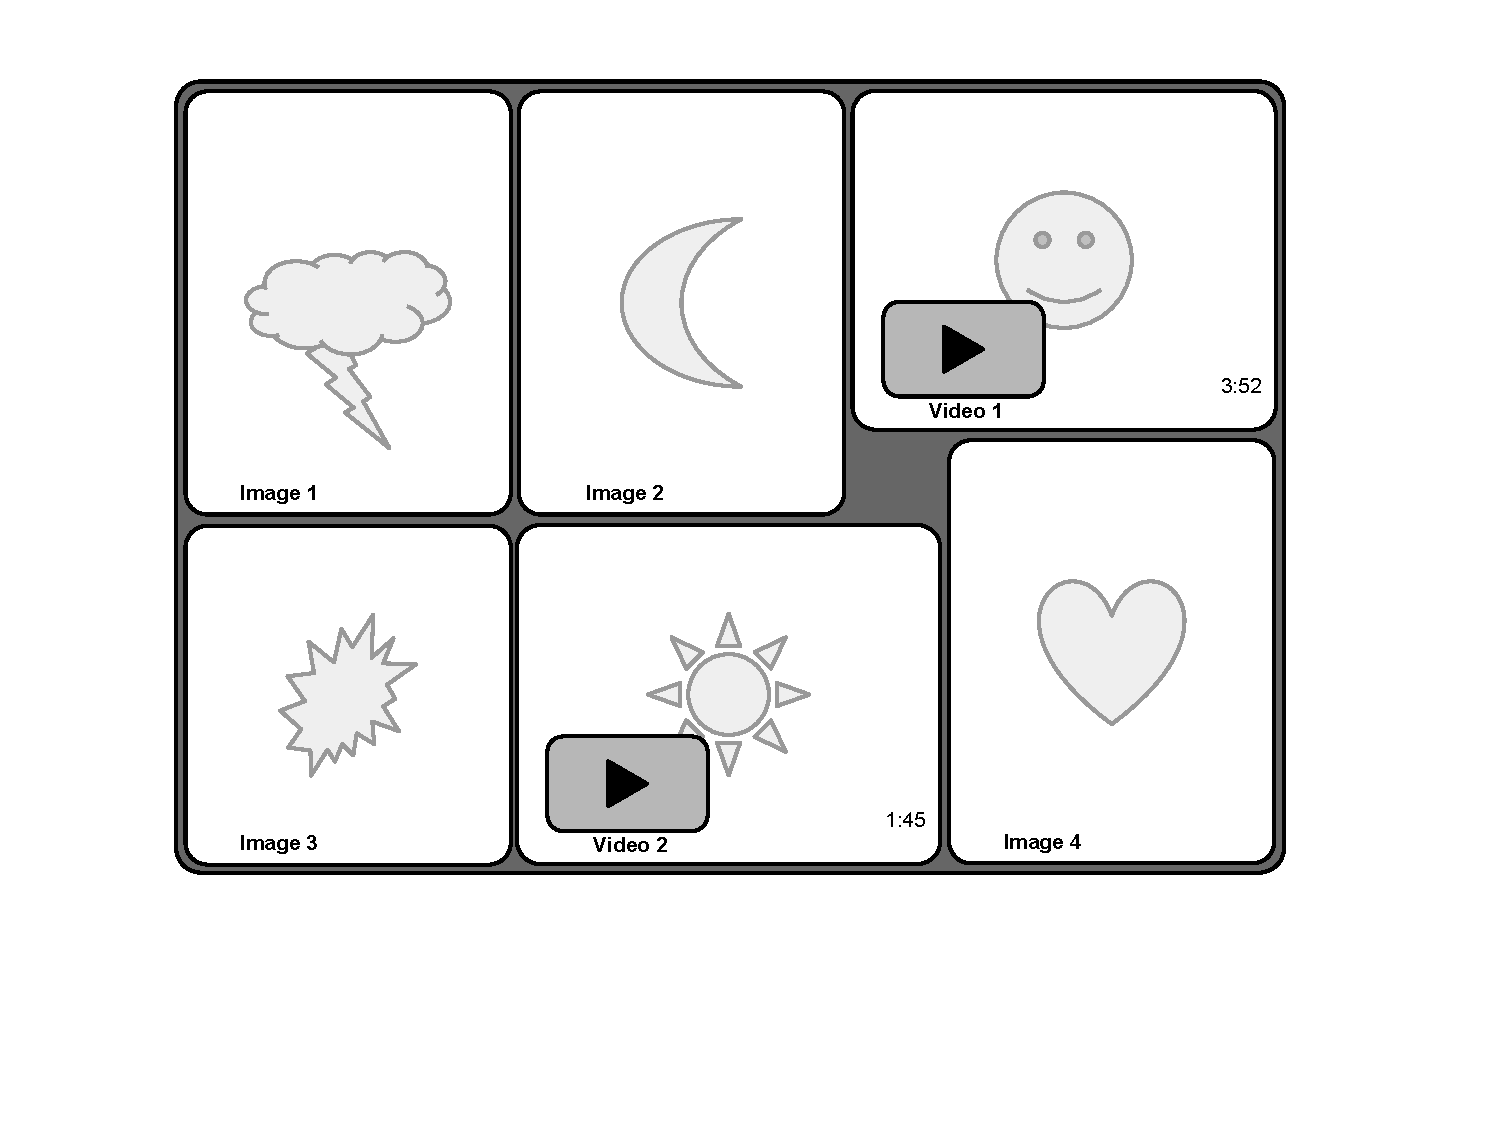
\includegraphics[trim=20mm 40mm 20mm 10mm, clip, width=0.75\columnwidth]{media-gallery.pdf}
\caption{Schematic media gallery with 4 images and 2 videos.}
\label{fig:media-gallery}
\end{figure}

\section{Related Work}
While enormous efforts have been made to extract those features
from media items and microposts on social networks in \emph{isolation},
to the best knowledge of the authors, remarkably less initiatives 
concern the extraction and the application
of all those features \emph{in combination}
for \emph{all} types of media items, including microposts.
In~\cite{Photo2011}, Sandhaus \emph{et al.}\ consider visual and
aesthetic features for the automatic creation of photo books.
Obrador \emph{et al.}\ use visual and aesthetic features
for a category-based approach to automatically assess
the aesthetic appeal of photographs~\cite{Photo2012}.
In~\cite{Playlist2006}, Knees \emph{et al.}\ use audial and textual
features for the automatic generation of music playlists.
Choudhury \emph{et al.}\ show in \cite{Sports2011} how social and textual
features can be used to achieve precise detection results 
of named entities and significant events in sports-related microposts.
In~\cite{YouTube2010}, Davidson \emph{et al.}\ show how visual,
textual, and social features can be used for personalized video recommendations.
A service called Storify~\cite{Storify2011} lets users manually combine
microposts, images, videos, and other elements onto one page for the purpose
of storytelling or summarizing an event,
and share stories permanently on the Web.
Finally, social networks present images and videos
often in grid-like galleries\footnote{\url{http://twitpic.com/904yka/full}}, sometimes scaled
based on the amount of comments.

\section{Media Item Ranking Criteria}
In this section, we describe several feature categories that can serve to rank
media items retrieved from social networks. 
We assume (and are working on) media item extractors that,
given event-related search terms,
extract raw binary media items and associated microposts
from multiple social networks.

\noindent \textbf{Visual}
This category regards the contents of images and videos.
We distinguish \emph{low-} and \emph{high-level} visual ranking criteria.
High-level criteria are, \emph{e.g.}, logo detection,
face recognition, and camera shot separation.
Low-level criteria are, \emph{e.g.}, size, resolution,
duration, geolocation, and time.
Via OCR, contained characters can be treated as textual features.

\noindent \textbf{Audial}
This category regards the audio track of videos.
\emph{High-level} ranking criteria are the presence or absence
of silence, music, speech, or a mixture thereof.
Similar to visual features before,
audial \emph{low-level} features are the average bit rate,
volume, possibly distorted areas, \emph{etc}.
Through audio-transcription, speech can be converted to a textual feature.

\noindent \textbf{Textual}
This category regards the microposts that accompany media items.
Typically, microposts provide a~description of media items.
Using named entity disambiguation tools,
textual content can be linked to LOD cloud concepts~\cite{Facebook2011}.

\noindent \textbf{Social}
This category regards social network effects like shares, mentions,
view counts, expressions of (dis)likes, user diversity, \emph{etc}.
Prior work~\cite{Khrouf2012} allows us to not only examine these effects
on a~\emph{single} social network,
but in a~\emph{network-agnostic} way across multiple social networks.

\noindent \textbf{Aesthetic}
This category regards the desired outcome after the ranking, \emph{i.e.},
the media gallery that illustrates a given event and its atmosphere.
Studies exist for the aesthetics of
automatic photo book layout~\cite{Photo2011},
photo aesthetics \emph{per se}~\cite{Photo2012},
video and music playlist generation~\cite{YouTube2010,Playlist2006},
however media gallery composition requires mixing video
\emph{and} image media items.

\section{Media Gallery Aesthetics}

\noindent \textbf{Definition}
A media gallery in our context is a compilation of images or videos
retrieved from social networks that are related to a given event.
Given a set $M = \{m_1,..., m_n\}$ of media items related to a certain event,
and given a ranking formula $f$,
the subset $M^\prime \subset M$
is the result after the application of $f$ to $M$: $f(M)=M^\prime$.
Each media item $m_i$ can either be an instance of video or image.
For each point $t_x$ on a timeline $T$, the state of the media gallery
at $t_x$ is defined for each media item $m_i$
as a set $S_x$ of $n$ tuples $s_{x,i}$, where
$s_{x,i}=\langle \mathit{left}$, $\mathit{top}$, $\mathit{width}$, $\mathit{height}$,
$\mathit{alpha}$, $\mathit{z\mbox{-}index}$, $\mathit{animation}$,
$\mathit{start}$, $\mathit{playing}$, $\mathit{volume} \rangle$.
The first 6~properties are defined as in CSS, the $\mathit{animation}$ property
allows for the definition of CSS transitions
and transformations as defined in~\cite{CSSTransitions2009,CSSTransforms2012},
the $\mathit{start}$ property defines the start time in a video.
A schematic media gallery at $t_x$ can be seen in \autoref{fig:media-gallery}.

\noindent \textbf{Audial aesthetics}
We recall the purpose of our media galleries:
to illustrate an event and its atmosphere.
Audial aesthetics thus consist of aspects like volume level normalization,
avoiding multiple videos playing music in parallel, smooth transitions, \emph{etc}.
We remark that through selective mixing of audio tracks
of event-related videos, ``noise clouds'' very characteristic
for the event atmosphere can be observed.

\noindent \textbf{Visual aesthetics}
Visual aesthetics are determined by the composition, \emph{i.e.},
the relation of images to videos \emph{globally}, \emph{per coherent scene},
and per \emph{point in time}.
In order not to overcharge the perceptive capacity
of viewers, the number of visible (moving) media items
at a time should be limited.
Depending on the event, a consistent or a contrasty overall
appearance of items may be desired, also for transitions.

\section{Conclusion}
We have introduced media item ranking criteria, and
aesthetic audial and visual principles for media galleries.
In the coming months, we will apply those principles
to a large collection of media items related to events,
and, via multivariate tests, measure user engagement
for different feature configurations.

\section{Evaluating Subjective Data}
Evaluating subjective data, like \emph{the} correct ranking
for a~set of media items, is a~challenging task.
For different users, there may be different optimal settings.
In order to get familiar with subjective evaluation techniques,
we have worked on a~side project with subjective data.

In May 2012, the Web search engine Google has introduced the so-called Knowledge Graph,
a~graph that understands real-world entities and their relationships to one another.
With the introduction of the Knowledge Graph, the search engine Google
has made a~significant paradigm shift towards \textit{``things, not strings''}~\cite{singhal2012},
as a~post on the official Google blog states.
Entities covered by the Knowledge Graph include landmarks, celebrities, cities, sports
teams, buildings, movies, celestial objects, works of art, and more.
The graph enhances Google search in three main ways:
by disambiguation of search queries,
by search log-based summarization of key facts,
and by explorative search suggestions.
With this work, we suggest a~fourth way of enhancing Web search:
through the addition of realtime coverage
of what people say about real-world entities on social networks.
We report on a~browser extension that seamlessly adds relevant microposts
from the social networking sites \googleplus, Facebook, and Twitter
in form of a~panel to Knowledge Graph entities.
In a~true Linked Data fashion, we interlink detected concepts in microposts
with Freebase entities, and evaluate our approach for both relevancy and usefulness.
The extension is freely available,
we invite the reader to reconstruct the examples of this work
to see how realtime opinions may have changed since time of writing.

Google News is a~news aggregator portal provided and operated by Google.
Earlier this year, a~new feature called \emph{realtime coverage}
was added to the portal~\cite{zuccarino2012}, providing signed in US \googleplus users
with the latest relevant posts from the \googleplus community for news stories.

We have implemented a~social network-agnostic approach
to add realtime coverage to Knowledge Graph results via a~browser extension.
The extension is freely available on the Chrome Web
Store\footnote{Knowledge Graph Socializer extension (\url{http://goo.gl/rzdVK})};
an also free Google API key is required.

\section{Methodology}
Chrome extensions are small software programs that users can install
to enrich their browsing experience.
Via so-called \emph{content scripts}, extensions can inject and modify the contents of Web pages.
We have implemented an extension that gets activated when a~user uses Google to search the Web.
If the extension detects that the current search engine results page
has an associated real-world entity in the Knowledge Graph,
first, it extracts the entity's name and Wikipedia URL.
Second, the extension performs full-text searches via the search APIs of
the popular social networking sites \googleplus, Twitter, and Facebook
and returns the top $n$ results (configurable) of each network.
Third, all microposts get analyzed and annotated via part-of-speech tagging.
For each (pair of) nouns, the Freebase search API is used
to link these strings with entities,
a~task commonly known as \emph{entity linking}~\cite{spitkovsky2012}.
We follow a~context-free, most frequent sense approach,
which, according to Agirre and Edmonds~\cite{agirre2007},
serves as a~surprisingly strong baseline,
an observation that we can confirm in our evaluation of micropost \emph{relevancy}
in \autoref{sec:relevancy}.
In a~final step, the resulting set of microposts is ordered chronologically
and attached in form of a~separate panel to the Knowledge Graph result.
A~screenshot with exemplary extension output for the entity
\emph{``Isabella Stewart Gardner Museum''} in Boston, MA,
is online\footnote{Screenshot of the extension (\url{http://twitpic.com/a8zgiq/full})}. 

\section{Evaluation}
For the evaluation, we have considered 100 microposts from 94 unique users,
out of which 72 microposts contained outbound links to overall 94 Web pages.
We have evaluated the extension on 21 real-world entities starting from the concept
\emph{``Boston,~MA''}, and then recursively following graph links to related concepts.
Our evaluation criteria were \emph{usefulness} of the information
contained in both the microposts and the potentially linked-to Web pages,
and the \emph{relevancy} of the microposts to the real-world entities in question.
We have calculated the Mean~Opinion Score (MOS)~\cite{mos1998} for both criteria.

Traditionally, MOS is used for conducting subjective evaluations
of telephony network transmission quality,
however, more recently, MOS has also found wider usage in the multimedia community
for evaluating \emph{per se} subjective things
like perceived quality from the users' perspective. 
Therefore, a~set of standard, subjective tests are conducted,
where a~number of users rate the quality of test samples
with scores ranging from 1 (worst) to 5 (best).
The actual MOS is then the arithmetic mean of all individual scores.
Given our intrinsically subjective evaluation criteria,
namely \emph{usefulness} and \emph{relevancy},
MOS provides a~meaningful way to judge the overall quality of our approach.

For \emph{relevancy}, the MOS was 4.38 out of 5.
For \emph{usefulness}, we have calculated a~MOS of 3.75 out of 5.
Our complete evaluation is available online\footnote{Evaluation (\url{http://goo.gl/dbvr4})}.
In the following, we provide an interpretation of the MOS results for both criteria.

\paragraph{Usefulness:}
The MOS of 3.75 suggests potential for improvement,
albeit the information from the microposts and linked-to Web pages
was overall still considered useful.
Positively rated revealed insights were, among others, recommended restaurants,
suggested things to do, scheduled future or past events,
special (not necessarily advertisement-like) offers, user-generated photos,
news articles, travel tips, or stories of everyday life.
On closer inspection, the microposts that teared down the \emph{usefulness} MOS
were in the majority of cases still rated relatively high for \emph{relevancy}.
We could track down the relevant but not useful microposts to three categories:
(i) long microposts (\googleplus, Facebook) that mentioned the concept somewhere,
but that were too long to skim,
(ii) so-called
@Replies\footnote{``What are @Replies and Mentions?'' (\url{http://goo.gl/Ge2RG})}
on Twitter that are messages to other Twitter users,
but that lack the context of the conversation, and finally
(iii) so-called native check-in messages on \googleplus,
together with shared Foursquare check-in messages on Twitter and Facebook
via connected user profiles\footnote{``Connecting/sharing to Facebook and Twitter'' (\url{http://goo.gl/NBuCr})}
that are geotagged (and thus relevant), however,
provide no other information besides the fact that a~user was at a~certain place.
By disregarding all three types of microposts, the MOS could be increased to 3.94.

\paragraph{Relevancy:} \label{sec:relevancy}
The high MOS of 4.38 shows that the microposts
were in the majority of cases considered very relevant.
On the one hand, this is due to the well-chosen titles of concepts in the graph,
which oftentimes are either unique enough (\emph{e.g.}, \emph{``\underline{Faneuil} Hall''}),
or on the other hand, include some sort of disambiguation aid
(\emph{e.g.}, \emph{``Museum of Science, \underline{Boston}''}).
In~\cite{spitkovsky2012}, Spitkovsky and Chang have collected
an extensive set of link titles for Wikipedia concepts
and shown that an entirely context-free approach
to linking strings with concepts does consistently well.
Together with the observation above, this justifies
our concept title-based full-text search approach on social networking sites,
reflected by the MOS.

\section{Future Work and Conclusion}
Each concept in the Knowledge Graph has a~unique identifier~\cite{thalhammer2012}.
Exploiting this fact and considering that Knowledge Graph results
have already been interlinked via \texttt{owl:sameAs}
with Freebase entities~\cite{glaser2012},
we can imagine a~comments archive of things people said about real-world entities.
The SIOC Ontology~\cite{breslin2005} by Breslin \emph{et al.}
provides an ideal vocabulary for such archive,
as both the context of the comments and their provenance can be described.
Taking it one step further, we can think of not only archiving user comments,
but also adding meaning to them~\cite{steiner2013},
which would allow for interesting use cases
like searching for places that are frequented by celebrities.

Concluding, in this work we have shown how realtime coverage
can be added to Knowledge Graph results via a~browser extension.
We have evaluated both the \emph{usefulness} and \emph{relevancy}
of the returned microposts and linked-to Web pages,
and have given an outlook on how via a~potentially enriched comments archive
about real-world entities, further use cases can be covered.
Through this work, we have demonstrated how the rather static, structured world
of real-world facts from the Knowledge Graph
(with facts like foundation date, opening hours, spouse, etc.),
can be successfully combined for fun and profit
with the rather dynamic, \emph{a~priori} unstructured world
of social network microposts.
ficken

\section{Ranking Formula}

\section{State of the Art}

\section{Evaluation}

\section{Conclusion}